\documentclass[12pt,twoside]{article}
\usepackage[dvipsnames]{xcolor}
\usepackage{tikz,graphicx,amsmath,amsfonts,amscd,amssymb,bm,cite,epsfig,epsf,url}
\usepackage[hang,flushmargin]{footmisc}
\usepackage[colorlinks=true,urlcolor=blue,citecolor=blue]{hyperref}
\usepackage{amsthm,multirow,wasysym,appendix}
\usepackage{array,subcaption} 
% \usepackage[small,bf]{caption}
\usepackage{bbm}
\usepackage{pgfplots}
\usetikzlibrary{spy}
\usepgfplotslibrary{external}
\usepgfplotslibrary{fillbetween}
\usetikzlibrary{arrows,automata}
\usepackage{thmtools}
\usepackage{blkarray} 
\usepackage{textcomp}
\usepackage[left=0.8in,right=1.0in,top=1.0in,bottom=1.0in]{geometry}
\usepackage{pifont}
\usepackage{tikz-qtree}

%% Probability operators and functions
%
% \def \P{\mathrm{P}}
\def \P{\mathrm{P}}
\def \E{\mathrm{E}}
\def \Var{\mathrm{Var}}
\let\var\Var
\def \Cov {\mathrm{Cov}} \let\cov\Cov
\def \MSE {\mathrm{MSE}} \let\mse\MSE
\def \sgn {\mathrm{sgn}}
\def \R {\mathbb{R}}
\def \C {\mathbb{C}}
\def \N {\mathbb{N}}
\def \Z {\mathbb{Z}}
\def \cV {\mathcal{V}}
\def \cS {\mathcal{S}}

\newcommand{\RR}{\ensuremath{\mathbb{R}}}

\DeclareMathOperator*{\argmin}{arg\,min}
\DeclareMathOperator*{\argmax}{arg\,max}
\newcommand{\red}[1]{\textcolor{red}{#1}}
\newcommand{\blue}[1]{\textcolor{blue}{#1}}
\newcommand{\green}[1]{\textcolor{ForestGreen}{ #1}}
\newcommand{\fuchsia}[1]{\textcolor{RoyalPurple}{ #1}}



%
%% Probability distributions
%
%\def \Bern    {\mathrm{Bern}}
%\def \Binom   {\mathrm{Binom}}
%\def \Exp     {\mathrm{Exp}}
%\def \Geom    {\mathrm{Geom}}
% \def \Norm    {\mathcal{N}}
%\def \Poisson {\mathrm{Poisson}}
%\def \Unif    {\mathrm {U}}
%
\DeclareMathOperator{\Norm}{\mathcal{N}}

\newcommand{\bdb}[1]{\textcolor{red}{#1}}

\newcommand{\ml}[1]{\mathcal{ #1 } }
\newcommand{\wh}[1]{\widehat{ #1 } }
\newcommand{\wt}[1]{\widetilde{ #1 } }
\newcommand{\conj}[1]{\overline{ #1 } }
\newcommand{\rnd}[1]{\tilde{ #1 } }
\newcommand{\rv}[1]{ \rnd{ #1}  }
\newcommand{\rM}{\rnd{ m}  }
\newcommand{\rx}{\rnd{ x}  }
\newcommand{\ry}{\rnd{ y}  }
\newcommand{\rz}{\rnd{ z}  }
\newcommand{\ra}{\rnd{ a}  }
\newcommand{\rb}{\rnd{ b}  }
\newcommand{\rt}{\rnd{ t}  }
\newcommand{\rs}{\rnd{ s}  }


\newcommand{\rpc}{\widetilde{ pc}  }
\newcommand{\rndvec}[1]{\vec{\rnd{#1}}}

\def \cnd {\, | \,}
\def \Id { I }
\def \J {\mathbf{1}\mathbf{1}^T}

\newcommand{\op}[1]{\operatorname{#1}}
\newcommand{\setdef}[2]{ := \keys{ #1 \; | \; #2 } }
\newcommand{\set}[2]{ \keys{ #1 \; | \; #2 } }
\newcommand{\sign}[1]{\op{sign}\left( #1 \right) }
\newcommand{\trace}[1]{\op{tr}\left( #1 \right) }
\newcommand{\tr}[1]{\op{tr}\left( #1 \right) }
\newcommand{\inv}[1]{\left( #1 \right)^{-1} }
\newcommand{\abs}[1]{\left| #1 \right|}
\newcommand{\sabs}[1]{| #1 |}
\newcommand{\keys}[1]{\left\{ #1 \right\}}
\newcommand{\sqbr}[1]{\left[ #1 \right]}
\newcommand{\sbrac}[1]{ ( #1 ) }
\newcommand{\brac}[1]{\left( #1 \right) }
\newcommand{\bbrac}[1]{\big( #1 \big) }
\newcommand{\Bbrac}[1]{\Big( #1 \Big)}
\newcommand{\BBbrac}[1]{\BIG( #1 \Big)}
\newcommand{\MAT}[1]{\begin{bmatrix} #1 \end{bmatrix}}
\newcommand{\sMAT}[1]{\left(\begin{smallmatrix} #1 \end{smallmatrix}\right)}
\newcommand{\sMATn}[1]{\begin{smallmatrix} #1 \end{smallmatrix}}
\newcommand{\PROD}[2]{\left \langle #1, #2\right \rangle}
\newcommand{\PRODs}[2]{\langle #1, #2 \rangle}
\newcommand{\der}[2]{\frac{\text{d}#2}{\text{d}#1}}
\newcommand{\pder}[2]{\frac{\partial#2}{\partial#1}}
\newcommand{\derTwo}[2]{\frac{\text{d}^2#2}{\text{d}#1^2}}
\newcommand{\ceil}[1]{\lceil #1 \rceil}
\newcommand{\Imag}[1]{\op{Im}\brac{ #1 }}
\newcommand{\Real}[1]{\op{Re}\brac{ #1 }}
\newcommand{\norm}[1]{\left|\left| #1 \right|\right| }
\newcommand{\norms}[1]{ \| #1 \|  }
\newcommand{\normProd}[1]{\left|\left| #1 \right|\right| _{\PROD{\cdot}{\cdot}} }
\newcommand{\normTwo}[1]{\left|\left| #1 \right|\right| _{2} }
\newcommand{\normTwos}[1]{ \| #1  \| _{2} }
\newcommand{\normZero}[1]{\left|\left| #1 \right|\right| _{0} }
\newcommand{\normTV}[1]{\left|\left| #1 \right|\right|  _{ \op{TV}  } }% _{\op{c} \ell_1} }
\newcommand{\normOne}[1]{\left|\left| #1 \right|\right| _{1} }
\newcommand{\normOnes}[1]{\| #1 \| _{1} }
\newcommand{\normOneTwo}[1]{\left|\left| #1 \right|\right| _{1,2} }
\newcommand{\normF}[1]{\left|\left| #1 \right|\right| _{\op{F}} }
\newcommand{\normLTwo}[1]{\left|\left| #1 \right|\right| _{\ml{L}_2} }
\newcommand{\normNuc}[1]{\left|\left| #1 \right|\right| _{\ast} }
\newcommand{\normOp}[1]{\left|\left| #1 \right|\right|  }
\newcommand{\normInf}[1]{\left|\left| #1 \right|\right| _{\infty}  }
\newcommand{\proj}[1]{\mathcal{P}_{#1} \, }
\newcommand{\diff}[1]{ \, \text{d}#1 }
\newcommand{\vc}[1]{\boldsymbol{\vec{#1}}}
\newcommand{\rc}[1]{\boldsymbol{#1}}
\newcommand{\vx}{\vec{x}}
\newcommand{\vy}{\vec{y}}
\newcommand{\vz}{\vec{z}}
\newcommand{\vu}{\vec{u}}
\newcommand{\vv}{\vec{v}}
\newcommand{\vb}{\vec{\beta}}
\newcommand{\va}{\vec{\alpha}}
\newcommand{\vaa}{\vec{a}}
\newcommand{\vbb}{\vec{b}}
\newcommand{\vg}{\vec{g}}
\newcommand{\vw}{\vec{w}}
\newcommand{\vh}{\vec{h}}
\newcommand{\vbeta}{\vec{\beta}}
\newcommand{\valpha}{\vec{\alpha}}
\newcommand{\vgamma}{\vec{\gamma}}
\newcommand{\veta}{\vec{\eta}}
\newcommand{\vnu}{\vec{\nu}}
\newcommand{\rw}{\rnd{w}}
\newcommand{\rvnu}{\vc{\nu}}
\newcommand{\rvv}{\rndvec{v}}
\newcommand{\rvw}{\rndvec{w}}
\newcommand{\rvx}{\rndvec{x}}
\newcommand{\rvy}{\rndvec{y}}
\newcommand{\rvz}{\rndvec{z}}
\newcommand{\rvX}{\rndvec{X}}


\newtheorem{theorem}{Theorem}[section]
% \declaretheorem[style=plain,qed=$\square$]{theorem}
\newtheorem{corollary}[theorem]{Corollary}
\newtheorem{definition}[theorem]{Definition}
\newtheorem{lemma}[theorem]{Lemma}
\newtheorem{remark}[theorem]{Remark}
\newtheorem{algorithm}[theorem]{Algorithm}

% \theoremstyle{definition}
%\newtheorem{example}[proof]{Example}
\declaretheorem[style=definition,qed=$\triangle$,sibling=definition]{example}
\declaretheorem[style=definition,qed=$\bigcirc$,sibling=definition]{application}

%
%% Typographic tweaks and miscellaneous
%\newcommand{\sfrac}[2]{\mbox{\small$\displaystyle\frac{#1}{#2}$}}
%\newcommand{\suchthat}{\kern0.1em{:}\kern0.3em}
%\newcommand{\qqquad}{\kern3em}
%\newcommand{\cond}{\,|\,}
%\def\Matlab{\textsc{Matlab}}
%\newcommand{\displayskip}[1]{\abovedisplayskip #1\belowdisplayskip #1}
%\newcommand{\term}[1]{\emph{#1}}
%\renewcommand{\implies}{\;\Rightarrow\;}



\begin{document}

\begin{center}
{\large{\textbf{Homework 6}} } \vspace{0.2cm}\\
Due Mar 19 at 11 pm
\\
\end{center}
Unless stated otherwise, justify any answers you give.
You can work in groups, but each
student must write their own solution based on their own
understanding of the problem.

When uploading your homework to Gradescope you will have to
select the relevant pages for each question.  Please submit each
problem on a separate page (i.e., 1a and~1b can be on the same page but 1
and 2 must be on different pages).  We understand that this may be
cumbersome but this is the best way for the grading team to grade your
homework assignments and provide feedback in a timely manner.  Failure
to adhere to these guidelines may result in a loss of points.
Note that it may take some time to
select the pages for your submission.  Please plan accordingly.  We
suggest uploading your assignment at least 30 minutes before the deadline
so you will have ample time to select the correct pages for your
submission.  If you are using \LaTeX, consider using the minted or
listings packages for typesetting code.  
\\

\begin{enumerate}

\item (Road renovation) 
A small town decides to renovate a 10-mile road in a small town. According to certain reports, there is a specific 2.5-mile section which is very dangerous. Completely renovating that section would use up all of the budget, so the engineer in charge of the renovation wants to make sure that this is a priority. She decides to perform a hypothesis test using the next 4 accidents reported on the road. Her null hypothesis is that the accidents are independent and uniformly distributed on the 10-mile road, which would imply that the \emph{dangerous} section is not that dangerous. The test statistic is the number of accidents that occur in the dangerous 2.5-mile section. The significance level is set to $\alpha := 0.05$.
\begin{enumerate}
\item Derive the p value function of the test for all possible values of the test statistic. 
\begin{itemize}
    \color{blue}
    \item the p value is the likelihood of observation a test stat that is larger than or equal to what we saw under the null hypothesis 
\item call $\Tilde{p}_i$ a Bernoulli rv representing if the ith accident occurred within the 2.5 mile section 
\item  under our null we think that $\Tilde{p}_i\sim \mathcal{U}(0,10)$ 
\item our test stat $\Tilde{t}=\Tilde{p}_1+\Tilde{p}_2+\Tilde{p}_3+\Tilde{p}_4$
\item under our null  we can think of the likelihood of each car crashing within the zone as independent, identically distributed Bernoulli's thus we can think of there sum ($\Tilde{t}$) as a distribute according to a binomial with parameters n=4 and $\theta$, where $\theta$ is the likelihood of crashing in the 2.5 mile danger zone
\item we know that this implies that our p-value function $pv(t)=P(\Tilde{t}_{\theta_{null}}\geq t)=\Sigma_{i=t}^{n}\begin{pmatrix}n\\i\end{pmatrix}(\theta_{null})^{i}(1-\theta_{null})^{n-i}$
\item we know that the stretch of rode we are interested in is 2.5 miles out of a total of 10 miles. thus under the null that a crash is equally likely to happen anywhere the likelihood of crashing in that zone is $\theta_{null}=\frac{2.5}{10}=\frac{1}{4}$
\item so plugging in we finally get $$pv(t)=P(\Tilde{t}_{\theta_{null}}\geq t)=\Sigma_{i=t}^{n}\begin{pmatrix}n\\i\end{pmatrix}(\theta_{null})^{i}(1-\theta_{null})^{n-i}=\Sigma_{i=t}^{4}\begin{pmatrix}4\\i\end{pmatrix}(\frac{1}{4})^{i}(\frac{3}{4})^{4-i}$$
\end{itemize}


\item What is the probability of a false positive?
\begin{itemize}
    \color{blue}
    \item the likelihood of a false positive as we showed in class is equal to $\alpha$so in this case it is $5\%$ 
\end{itemize}
\item Let $\theta$ denote the probability that an accident occurs in the \emph{dangerous} section. Plot the power function of the test as a function of $\theta$ under the assumption that accidents occur independently. 
\begin{itemize}
    \color{blue}
    \item  the power function is a function that maps any given effect size $\theta$ to our likely hood of rejecting the null hypothesis. ie $$pow(\theta)=P(pv(t_{\theta})\leq \alpha) $$
\item so first things first we need to find our $\tau_{threshold}$ which is the minimum test stat value at which we will reject the null hypothesis for a given $\alpha$ that is $$\tau_{threshold}=min_{1\leq \tau\leq n}\{\tau:P(\Tilde{t}\geq \tau)\leq \alpha\}=min_{1\leq \tau\leq n}\{\tau:\Sigma_{i=t}^{n}\begin{pmatrix}n\\i\end{pmatrix}(\theta)^{i}(1-\theta)^{n-i}\leq \alpha\}$$$$=min_{1\leq \tau\leq n}\{\tau:\Sigma_{i=t}^{4}\begin{pmatrix}4\\i\end{pmatrix}(\frac{1}{4})^{i}(\frac{3}{4})^{4-i}\leq \alpha\}$$
\item for a fixed value of $n=4$ and $\alpha=.05$ we can compute $pv(3)=0.05078125\aprox 3$, but a bit above so i am going with 4. 
\item so we can write our power function as for any $\theta$ as  $$pow(\theta)=P(pv(t_{\theta})\leq \alpha)=P(t_{\theta}\leq \tau_{threshold})= \Sigma_{i=\tau_{threshold}}
^{4}\begin{pmatrix}4\\i\end{pmatrix}(\theta)^{i}(1-\theta)^{4-i}$$ $$=\begin{pmatrix}4\\4\end{pmatrix}(\theta)^{4}(1-\theta)^{0}=(\theta)^4$$

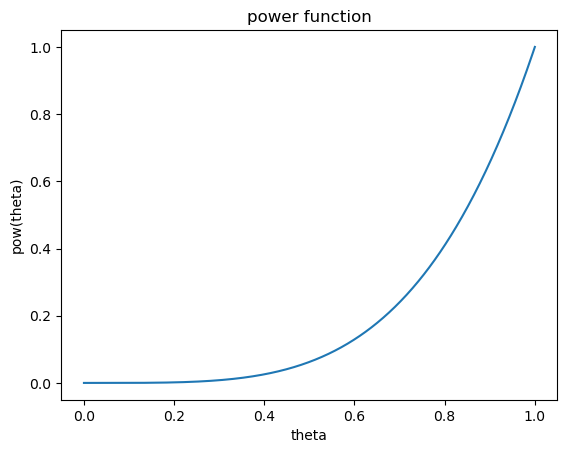
\includegraphics[widht=10cm]{homework/homework_6/immages/output.png}
\item above is a graph of the power function 

\end{itemize}
\item What is the minimum value of $\theta$ for which the probability of a true positive is at least 50\%?
\begin{itemize}
    \color{blue}
    \item recall that as we showed above $pow(\theta)=\theta^4$ thus we can find $\theta_{.5}$ such that $pow(\theta_{.5})=.5=(\theta_{.5})^{4}$ meaning that $\theta_{.05}=\sqrt[4]{0.5}$
\end{itemize}
\end{enumerate}
\newpage



\item (Computer component) A computer manufacturer wants to make sure that a certain component will last on average more than a year. They decide to apply a hypothesis test, where the null hypothesis is that the average duration is less than a year. The data correspond to $n$ instances of the component, which can be assumed to be independent. The test statistic is the minimum duration of the $n$ instances. If the time until the component fails is modeled using an exponential distribution, what is the power function of the test as a function of the exponential parameter $\lambda$ and the significance level $\alpha$? What is the power at $\lambda = 1$ and what is its limit as $\lambda \rightarrow 0$?
\begin{itemize}
    \color{blue}
    \item call $\Tilde{c}_i$ the time until the ith component fails. we know $\Tilde{c}_i\sim exp(\lambda)$
    \item further we know that the test stat is the minimum fail time of the n computers. thus $\Tilde{t}_{\lambda}=min(\Tilde{c}_1...\Tilde{c}_n)$
    \item so we can see that $P(\Tilde{t}_{\lambda}\geq t)=P(\Tilde{c}_1,...\Tilde{c}_n\geq n)$ further given that the components are indecent this can be expressed as $P(\Tilde{t}_{\lambda}\geq t)=P(\Tilde{c}_1,...\Tilde{c}_n\geq t)=P(\Tilde{c}_1\geq t)*..*P(\Tilde{c}_{n}\leq t)=e^{-\lambda t n}$
\item thus we can see that $\Tilde{t}_{\lambda}\sim exp(\lambda n)$
\item so if we think of t in terms of continuous quantities of days we have $\lambda$ represents the mean number of times a component breaks down within an interval. so if we think of the interval in years our null hypothesis is that $\lambda \in \lambda_{null}=(0,1)$

\item so we first must look at our p-value function $sup_{\lambda\in (0,1)}pv(t)=sup_{\lambda\in (0,1)}P(\Tilde{t}_{\lambda}\geq t)=sup_{\lambda\in (0,1)}1-
F_{\Tilde{t}_{\lambda}}(t)=sup_{\lambda\in (0,1)}1-1+e^{-\lambda n t}=sup_{\lambda\in (0,1)}e^{-\lambda n t}$
\item that function is decreasing in $\lambda$ so we would pick $\lambda$ as small as possible
\item now we need to find our $\tau_{thresohold}$ 
\item and further with out making any specific assumptions about $\lambda$ we can solve for our $\tau_{threshold}$ as     $\tau_{threshold}=min_{0\leq \tau}\{\tau:P(\Tilde{t}_{\theta}\geq \tau)\leq \alpha\}=min_{0\leq \tau}\{\tau:1-F_{\Tilde{t}_{\theta}}(t)\leq \alpha\}=min_{0\leq \tau}\{\tau:e^{-\lambda t}\leq \alpha\}=min_{0\leq \tau}\{\tau:-\lambda t\leq log(\alpha)\}=min_{0\leq \tau}\{\tau:{t}\geq\frac{ log(\alpha)}{\lambda}\}$ 
    \item thus we can express our power function as a function of $\lambda, \alpha $ as $pow(\lambda, \alpha)=P(pv(t_{\lambda})\leq \alpha)=P(t_{\lambda}\geq \tau_{threshold}(\alpha, \lambda))=1-F_{\Tilde{t}_{\lambda}(\tau_{threshold}}(\lambda ,\alpha))= e^{-\lambda \tau_{threshold}(\alpha, \lambda)}=e^{-\lambda * min_{0\leq \tau}\{\tau:{t}\geq\frac{-log(\alpha)}{\lambda}\}}$
    \item at $\lambda=1$ this becomes $pow(\lambda, \alpha)=P(pv(t_{\lambda})\leq \alpha)=P(t_{\lambda}\geq \tau_{threshold}(\alpha, \lambda))=1-F_{\Tilde{t}_{\lambda}(\tau_{threshold}}(\lambda ,\alpha))= e^{-\lambda \tau_{threshold}(\alpha, \lambda)t}=e^{ -\lambda * min_{0\leq \tau}\{\tau:{t}\geqlog(\alpha)\}t}=e^{-\lambda log(\alpha) t}$ but i mean this must be wrong? the exponential function is lower bounded by 1 so it cant really be understood as a probability? 
    \\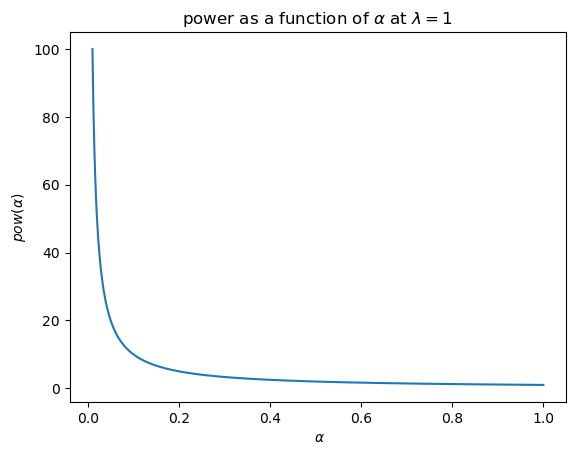
\includegraphics[width=10cm]{homework/homework_6/immages/question_2_1.png}
    \\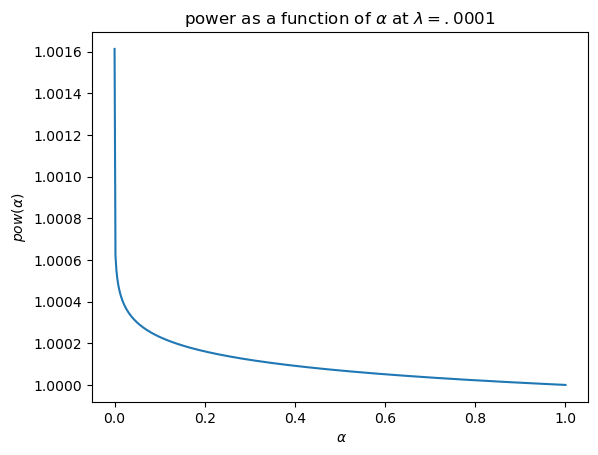
\includegraphics[width=10cm]{homework/homework_6/immages/question_2_2.png}
    \\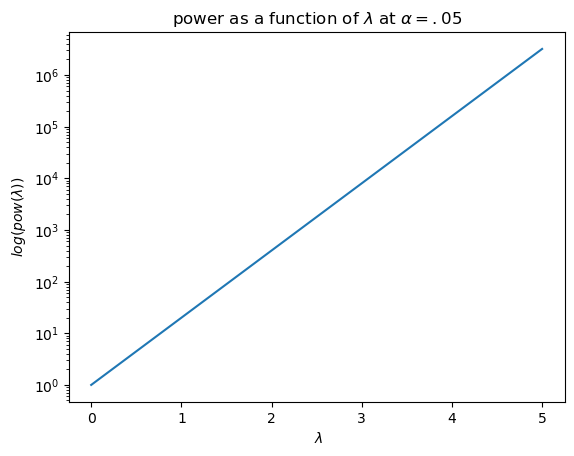
\includegraphics[width=10cm]{homework/homework_6/immages/question_2_3.png}
\end{itemize}
\newpage




\item (Tom Brady and hurricanes) 
The table shows in what years between 2001 and 2020 Tom Brady won the Super Bowl (top row) and there was at least one Category 5 hurricane in the North Atlantic Ocean (bottom row).\\
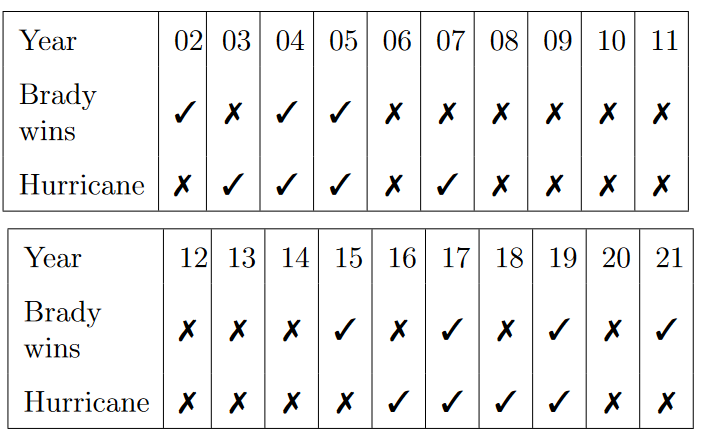
\includegraphics[width=10cm]{homework/homework_6/immages/Screenshot 2023-03-19 at 16-23-37 hw6.pdf.png}
\begin{enumerate}
\item Compute the p value of a one-tailed two-sample z test, where the null hypothesis is that hurricanes have the same distribution when Brady wins and when he doesn't. 
\begin{itemize}
    \color{blue}
    \item we were not explicitly given a test stat but lets call $\Tilde{y}_{i}$ a Bernoulli variable representing if there was hurricane that year and have our test stat be the difference in average number of hurricanes over the years tome Brady wins and did not win the super bowl that is $\Tilde{t}=\frac{1}{n_A}\Sigma_{i\in A}\Tilde{y}_i-\frac{1}{n_B}\Sigma_{i\in B}\Tilde{y}_i$
    
    \item we estimate $\theta_{null}$ as $\theta_{null}=\frac{\text{number of times there is a hurricane}}{\text{number of years}}=\frac{8}{20}=\frac{2}{5}$
    \item then we can estimate the $\sigma_{null}=\sqrt{\theta_{null}(1-\theta_{null})(\frac{1}{n_A}+\frac{1}{n_B})}$ where $n_A$ is the number of times Brady won a super bowl (7) and $n_B$ is the number of times Brady did not win a super brawl $(13)$thus $\sigma_{null}=\sqrt{\theta_{null}(1-\theta_{null})(\frac{1}{n_A}+\frac{1}{n_B})}=\sqrt{\frac{2}{5}\frac{3}{5}(\frac{1}{7}+\frac{1}{13})}=0.22966770070528583$
    \item so our $\Tilde{t}_{tail-1}\approx.229\Tilde{z}$ where $\Tilde{z}\sim \mathcal{N}(0,1)$
    \item thus we can find $Pv(t)=P(\Tilde{t}_{1-tail}\geq t)=P(\Tilde{z}\geq \frac{t}{0.229})$ \item so we can find the test stat of our data  ${t}_{data}=\frac{4}{7}-\frac{4}{13}\approx .263$
    \item so thus we can see that $pv({t}_{data})=P(\Tilde{t}\geq {t}_{data})=P(\Tilde{z}\geq \frac{.263}{.229})\approx0.12541442496047006$
    \item so we fail to reject the null in this case. 
\end{itemize}

\item If the p value had been extremely small, would this be convincing evidence that hurricanes occur more often when Brady wins? Justify your answer.
\begin{itemize}
    \color{blue}
    \item no this would not convince me of that conclusion as the assumptions of our test we clearly not met. We do not have large enough sample to reasonably believe that they will be approximately Gaussian 
    \item also from a logical perspective Tom Brady winning the super bowl and there being a hurricane are clearly unrelated. 
\end{itemize}
\end{enumerate}
\newpage





\item (Disease prevalence)
Doctors would like to research the prevalence of a disease of a certain population. They collected some patients records that can be interpreted as samples from that population. The table in \texttt{ehr.csv} records the diagnosis (\textit{Dx}). Specifically, they choose the two null hypotheses below. For each null hypothesis, choose a hypothesis test and a test statistic and compute the corresponding p-value. 
\begin{enumerate}
\item The prevalence of this disease is greater than 0.3.
\begin{itemize}
    \color{blue}
    \item they are interested in the prevalence of the disease.
    \item call $\theta$ the prevalence of the disease 
    \item the null is in this case is $\theta\in \Theta_{null}=(.3,1]$
    \item so let $\Tilde{x}_i$ be a Bernoulli rv with parameter $\theta$ which takes value one if a person has the disease, which we assume to be iid. 
    \item so lets have our test stat under so $\theta$ be $\Tilde{t}_{\theta}=\frac{1}{n}\Sigma_{i=1}^{n}\Tilde{x}_i$
    \item this is a sum of iid random variables and we know we have 7212 samples in our data thus it is reasonable to assume our data is approximately Gaussian that is $\Tilde{t}_{\theta}\sim \mathcal{N}(\theta_{null}, \frac{\theta_{null}(1-\theta_{null}}{n}))$
    \item so thus our p value function is $pv(t)=sup_{\theta\in \Theta_{null}}P(\Tilde{t}_{\theta}\geq t)=sup_{\theta\in \Theta_{null}}P(\Tilde{t}_{\theta}\geq t)=P(\Tilde{t}_{.3}\geq t)=\int_{i=t}^{\infty}f_{\Tilde{t}_{.3}}(t)dt$ 
    \item we can find the mean prevalence in the population as our observed test stat in the data as $t_{data}=0.3068071537501733$
    \item and find that the p-value of our data is $pv(t_{data})=0.10355045769142213$
\end{itemize}


\item Men and women have the same prevalence.
\begin{itemize}
    \color{blue}
\item call $\theta$ the  prevalence of the disease 
    \item so let $\Tilde{x}_i$ be a Bernoulli rv with parameter $\theta$ which takes value one if a person has the disease, which we assume to be iid. 
    \item so let us break our data in two groups. group A consisting of the men in the sample, and group b consisting of the women in the sample
    \item so lets do a two sided test and have our test stat under $\theta$ be $\Tilde{t}_{\theta}=|\frac{1}{_An}\Sigma_{i\in A}\Tilde{x}_i-\frac{1}{_An}\Sigma_{i\in A}\Tilde{x}_i|$
    \item this is a sum of scaled  iid random variables and we know we have 7212 samples in our data thus it is reasonable to assume our data is approximately Gaussian that is $\Tilde{t}_{\theta}\sim \mathcal{N}(0, {\theta_{null}(1-\theta_{null}})({\frac{1}{n_A}+\frac{1}{n_B}}))$ 
    \item from the data we can find $\theta_{null}=\frac{\text{number of people with the disease}}{n}=0.3068071537501733$
    \item in our data the two sided test stat was $t_{data}=0.23929310619328134$
    \item and so our p-value is $pv(t_{data})=P(\Tilde{t}_{null}\leq t_{data})=\int_{t=t_{data}}^{\infty}f_{\Tilde{t}_{\theta_{null}}}(t)dt\approx 0$
\end{itemize}

\end{enumerate}

\end{enumerate}
\end{document}
